% Options for packages loaded elsewhere
\PassOptionsToPackage{unicode}{hyperref}
\PassOptionsToPackage{hyphens}{url}
\documentclass[
]{article}
\usepackage{xcolor}
\usepackage[margin=1in]{geometry}
\usepackage{amsmath,amssymb}
\setcounter{secnumdepth}{-\maxdimen} % remove section numbering
\usepackage{iftex}
\ifPDFTeX
  \usepackage[T1]{fontenc}
  \usepackage[utf8]{inputenc}
  \usepackage{textcomp} % provide euro and other symbols
\else % if luatex or xetex
  \usepackage{unicode-math} % this also loads fontspec
  \defaultfontfeatures{Scale=MatchLowercase}
  \defaultfontfeatures[\rmfamily]{Ligatures=TeX,Scale=1}
\fi
\usepackage{lmodern}
\ifPDFTeX\else
  % xetex/luatex font selection
\fi
% Use upquote if available, for straight quotes in verbatim environments
\IfFileExists{upquote.sty}{\usepackage{upquote}}{}
\IfFileExists{microtype.sty}{% use microtype if available
  \usepackage[]{microtype}
  \UseMicrotypeSet[protrusion]{basicmath} % disable protrusion for tt fonts
}{}
\makeatletter
\@ifundefined{KOMAClassName}{% if non-KOMA class
  \IfFileExists{parskip.sty}{%
    \usepackage{parskip}
  }{% else
    \setlength{\parindent}{0pt}
    \setlength{\parskip}{6pt plus 2pt minus 1pt}}
}{% if KOMA class
  \KOMAoptions{parskip=half}}
\makeatother
\usepackage{color}
\usepackage{fancyvrb}
\newcommand{\VerbBar}{|}
\newcommand{\VERB}{\Verb[commandchars=\\\{\}]}
\DefineVerbatimEnvironment{Highlighting}{Verbatim}{commandchars=\\\{\}}
% Add ',fontsize=\small' for more characters per line
\usepackage{framed}
\definecolor{shadecolor}{RGB}{248,248,248}
\newenvironment{Shaded}{\begin{snugshade}}{\end{snugshade}}
\newcommand{\AlertTok}[1]{\textcolor[rgb]{0.94,0.16,0.16}{#1}}
\newcommand{\AnnotationTok}[1]{\textcolor[rgb]{0.56,0.35,0.01}{\textbf{\textit{#1}}}}
\newcommand{\AttributeTok}[1]{\textcolor[rgb]{0.13,0.29,0.53}{#1}}
\newcommand{\BaseNTok}[1]{\textcolor[rgb]{0.00,0.00,0.81}{#1}}
\newcommand{\BuiltInTok}[1]{#1}
\newcommand{\CharTok}[1]{\textcolor[rgb]{0.31,0.60,0.02}{#1}}
\newcommand{\CommentTok}[1]{\textcolor[rgb]{0.56,0.35,0.01}{\textit{#1}}}
\newcommand{\CommentVarTok}[1]{\textcolor[rgb]{0.56,0.35,0.01}{\textbf{\textit{#1}}}}
\newcommand{\ConstantTok}[1]{\textcolor[rgb]{0.56,0.35,0.01}{#1}}
\newcommand{\ControlFlowTok}[1]{\textcolor[rgb]{0.13,0.29,0.53}{\textbf{#1}}}
\newcommand{\DataTypeTok}[1]{\textcolor[rgb]{0.13,0.29,0.53}{#1}}
\newcommand{\DecValTok}[1]{\textcolor[rgb]{0.00,0.00,0.81}{#1}}
\newcommand{\DocumentationTok}[1]{\textcolor[rgb]{0.56,0.35,0.01}{\textbf{\textit{#1}}}}
\newcommand{\ErrorTok}[1]{\textcolor[rgb]{0.64,0.00,0.00}{\textbf{#1}}}
\newcommand{\ExtensionTok}[1]{#1}
\newcommand{\FloatTok}[1]{\textcolor[rgb]{0.00,0.00,0.81}{#1}}
\newcommand{\FunctionTok}[1]{\textcolor[rgb]{0.13,0.29,0.53}{\textbf{#1}}}
\newcommand{\ImportTok}[1]{#1}
\newcommand{\InformationTok}[1]{\textcolor[rgb]{0.56,0.35,0.01}{\textbf{\textit{#1}}}}
\newcommand{\KeywordTok}[1]{\textcolor[rgb]{0.13,0.29,0.53}{\textbf{#1}}}
\newcommand{\NormalTok}[1]{#1}
\newcommand{\OperatorTok}[1]{\textcolor[rgb]{0.81,0.36,0.00}{\textbf{#1}}}
\newcommand{\OtherTok}[1]{\textcolor[rgb]{0.56,0.35,0.01}{#1}}
\newcommand{\PreprocessorTok}[1]{\textcolor[rgb]{0.56,0.35,0.01}{\textit{#1}}}
\newcommand{\RegionMarkerTok}[1]{#1}
\newcommand{\SpecialCharTok}[1]{\textcolor[rgb]{0.81,0.36,0.00}{\textbf{#1}}}
\newcommand{\SpecialStringTok}[1]{\textcolor[rgb]{0.31,0.60,0.02}{#1}}
\newcommand{\StringTok}[1]{\textcolor[rgb]{0.31,0.60,0.02}{#1}}
\newcommand{\VariableTok}[1]{\textcolor[rgb]{0.00,0.00,0.00}{#1}}
\newcommand{\VerbatimStringTok}[1]{\textcolor[rgb]{0.31,0.60,0.02}{#1}}
\newcommand{\WarningTok}[1]{\textcolor[rgb]{0.56,0.35,0.01}{\textbf{\textit{#1}}}}
\usepackage{longtable,booktabs,array}
\usepackage{calc} % for calculating minipage widths
% Correct order of tables after \paragraph or \subparagraph
\usepackage{etoolbox}
\makeatletter
\patchcmd\longtable{\par}{\if@noskipsec\mbox{}\fi\par}{}{}
\makeatother
% Allow footnotes in longtable head/foot
\IfFileExists{footnotehyper.sty}{\usepackage{footnotehyper}}{\usepackage{footnote}}
\makesavenoteenv{longtable}
\usepackage{graphicx}
\makeatletter
\newsavebox\pandoc@box
\newcommand*\pandocbounded[1]{% scales image to fit in text height/width
  \sbox\pandoc@box{#1}%
  \Gscale@div\@tempa{\textheight}{\dimexpr\ht\pandoc@box+\dp\pandoc@box\relax}%
  \Gscale@div\@tempb{\linewidth}{\wd\pandoc@box}%
  \ifdim\@tempb\p@<\@tempa\p@\let\@tempa\@tempb\fi% select the smaller of both
  \ifdim\@tempa\p@<\p@\scalebox{\@tempa}{\usebox\pandoc@box}%
  \else\usebox{\pandoc@box}%
  \fi%
}
% Set default figure placement to htbp
\def\fps@figure{htbp}
\makeatother
\setlength{\emergencystretch}{3em} % prevent overfull lines
\providecommand{\tightlist}{%
  \setlength{\itemsep}{0pt}\setlength{\parskip}{0pt}}
\usepackage{bookmark}
\IfFileExists{xurl.sty}{\usepackage{xurl}}{} % add URL line breaks if available
\urlstyle{same}
\hypersetup{
  pdftitle={Homework1},
  hidelinks,
  pdfcreator={LaTeX via pandoc}}

\title{Homework1}
\author{}
\date{\vspace{-2.5em}2026-02-23}

\begin{document}
\maketitle

\section{Question 1}\label{question-1}

I am going to add packages as needed, allows me to keep better track of
questions and solving procedures.

\begin{Shaded}
\begin{Highlighting}[]
\FunctionTok{library}\NormalTok{(glmnet)  }
\FunctionTok{library}\NormalTok{(dplyr)  }
\end{Highlighting}
\end{Shaded}

\subsubsection{1) Working Directory}\label{working-directory}

\begin{Shaded}
\begin{Highlighting}[]
\FunctionTok{setwd}\NormalTok{(}\StringTok{"/Users/karolinawiesiolek/Desktop/Mailman Spring 2026/DSII/HW1/Homework\_1"}\NormalTok{)}

\CommentTok{\# sanity check: shows what R thinks the folder is}
\FunctionTok{getwd}\NormalTok{()}
\end{Highlighting}
\end{Shaded}

\begin{verbatim}
## [1] "/Users/karolinawiesiolek/Desktop/Mailman Spring 2026/DSII/HW1/Homework_1"
\end{verbatim}

\begin{Shaded}
\begin{Highlighting}[]
\CommentTok{\# sanity check: shows what files R sees inside this folder}
\FunctionTok{list.files}\NormalTok{()}
\end{Highlighting}
\end{Shaded}

\begin{verbatim}
##  [1] "dictionary.txt"        "Homework_1 copy.Rproj" "Homework_1.html"      
##  [4] "Homework_1.Rmd"        "Homework_1.Rproj"      "Homework_1tryout.log" 
##  [7] "Homework_1tryout.Rmd"  "Homework_1tryout.tex"  "housing_test.csv"     
## [10] "housing_training.csv"  "README copy.md"        "README.md"
\end{verbatim}

\textbf{Explanation} - \texttt{setwd(...)} tells R ``this is the folder
where my files live.'' - \texttt{list.files()} is your fastest way to
confirm the exact filenames (spaces, underscores, ``(1)'', etc.).

\begin{center}\rule{0.5\linewidth}{0.5pt}\end{center}

\subsubsection{2) Read training + test data (robust to filename
variations)}\label{read-training-test-data-robust-to-filename-variations}

This chunk tries to find the train/test/dictionary files even if they
have slightly different names (like ``training (1).csv'').

\begin{Shaded}
\begin{Highlighting}[]
\CommentTok{\# {-}{-}{-} Helper function: find a file by keyword pattern {-}{-}{-}}
\NormalTok{pick\_file }\OtherTok{\textless{}{-}} \ControlFlowTok{function}\NormalTok{(pattern) \{}
\NormalTok{  f }\OtherTok{\textless{}{-}} \FunctionTok{list.files}\NormalTok{(}\AttributeTok{pattern =}\NormalTok{ pattern, }\AttributeTok{ignore.case =} \ConstantTok{TRUE}\NormalTok{)}
  \ControlFlowTok{if}\NormalTok{ (}\FunctionTok{length}\NormalTok{(f) }\SpecialCharTok{==} \DecValTok{0}\NormalTok{) }\FunctionTok{stop}\NormalTok{(}\StringTok{"Could not find file matching pattern: "}\NormalTok{, pattern)}
\NormalTok{  f[}\DecValTok{1}\NormalTok{]  }\CommentTok{\# take the first match}
\NormalTok{\}}

\NormalTok{train\_file }\OtherTok{\textless{}{-}} \FunctionTok{pick\_file}\NormalTok{(}\StringTok{"train|training"}\NormalTok{)}
\NormalTok{test\_file  }\OtherTok{\textless{}{-}} \FunctionTok{pick\_file}\NormalTok{(}\StringTok{"test"}\NormalTok{)}
\NormalTok{dict\_file  }\OtherTok{\textless{}{-}} \FunctionTok{pick\_file}\NormalTok{(}\StringTok{"dict|dictionary"}\NormalTok{)}

\NormalTok{train\_raw }\OtherTok{\textless{}{-}} \FunctionTok{read.csv}\NormalTok{(train\_file, }\AttributeTok{stringsAsFactors =} \ConstantTok{FALSE}\NormalTok{, }\AttributeTok{check.names =} \ConstantTok{FALSE}\NormalTok{)}
\NormalTok{test\_raw  }\OtherTok{\textless{}{-}} \FunctionTok{read.csv}\NormalTok{(test\_file,  }\AttributeTok{stringsAsFactors =} \ConstantTok{FALSE}\NormalTok{, }\AttributeTok{check.names =} \ConstantTok{FALSE}\NormalTok{)}

\FunctionTok{dim}\NormalTok{(train\_raw)}
\end{Highlighting}
\end{Shaded}

\begin{verbatim}
## [1] 1440   26
\end{verbatim}

\begin{Shaded}
\begin{Highlighting}[]
\FunctionTok{dim}\NormalTok{(test\_raw)}
\end{Highlighting}
\end{Shaded}

\begin{verbatim}
## [1] 959  26
\end{verbatim}

\begin{Shaded}
\begin{Highlighting}[]
\FunctionTok{names}\NormalTok{(train\_raw)[}\DecValTok{1}\SpecialCharTok{:}\DecValTok{10}\NormalTok{]}
\end{Highlighting}
\end{Shaded}

\begin{verbatim}
##  [1] "Gr_Liv_Area"     "First_Flr_SF"    "Second_Flr_SF"   "Total_Bsmt_SF"  
##  [5] "Low_Qual_Fin_SF" "Wood_Deck_SF"    "Open_Porch_SF"   "Bsmt_Unf_SF"    
##  [9] "Mas_Vnr_Area"    "Garage_Cars"
\end{verbatim}

\textbf{Explanation} - \texttt{pick\_file()} searches your folder using
a regex pattern. - \texttt{read.csv(...,\ check.names\ =\ FALSE)}
prevents R from silently changing column names (important because your
response is \texttt{"Sale\ price"} with a space). -
\texttt{stringsAsFactors\ =\ FALSE} keeps character columns as character
(we'll handle dummy coding ourselves).

\begin{center}\rule{0.5\linewidth}{0.5pt}\end{center}

\subsubsection{3) Standardize the response column
name}\label{standardize-the-response-column-name}

Your homework says the response column is \texttt{"Sale\ price"}, but
sometimes it appears as \texttt{"Sale\_Price"} or \texttt{"SalePrice"}.
This code detects it and renames it to \texttt{SalePrice} in both
train/test.

\begin{Shaded}
\begin{Highlighting}[]
\NormalTok{resp\_candidates }\OtherTok{\textless{}{-}} \FunctionTok{c}\NormalTok{(}\StringTok{"Sale price"}\NormalTok{, }\StringTok{"Sale\_Price"}\NormalTok{, }\StringTok{"SalePrice"}\NormalTok{, }\StringTok{"sale\_price"}\NormalTok{, }\StringTok{"Sale Price"}\NormalTok{)}

\NormalTok{resp\_train }\OtherTok{\textless{}{-}}\NormalTok{ resp\_candidates[resp\_candidates }\SpecialCharTok{\%in\%} \FunctionTok{names}\NormalTok{(train\_raw)][}\DecValTok{1}\NormalTok{]}
\NormalTok{resp\_test  }\OtherTok{\textless{}{-}}\NormalTok{ resp\_candidates[resp\_candidates }\SpecialCharTok{\%in\%} \FunctionTok{names}\NormalTok{(test\_raw)][}\DecValTok{1}\NormalTok{]}

\FunctionTok{stopifnot}\NormalTok{(}\SpecialCharTok{!}\FunctionTok{is.na}\NormalTok{(resp\_train), }\SpecialCharTok{!}\FunctionTok{is.na}\NormalTok{(resp\_test))}

\NormalTok{train\_raw }\OtherTok{\textless{}{-}}\NormalTok{ train\_raw }\SpecialCharTok{\%\textgreater{}\%} \FunctionTok{rename}\NormalTok{(}\AttributeTok{SalePrice =} \FunctionTok{all\_of}\NormalTok{(resp\_train))}
\NormalTok{test\_raw  }\OtherTok{\textless{}{-}}\NormalTok{ test\_raw  }\SpecialCharTok{\%\textgreater{}\%} \FunctionTok{rename}\NormalTok{(}\AttributeTok{SalePrice =} \FunctionTok{all\_of}\NormalTok{(resp\_test))}

\FunctionTok{summary}\NormalTok{(train\_raw}\SpecialCharTok{$}\NormalTok{SalePrice)}
\end{Highlighting}
\end{Shaded}

\begin{verbatim}
##    Min. 1st Qu.  Median    Mean 3rd Qu.    Max. 
##   52000  130000  159000  177568  207000  755000
\end{verbatim}

\textbf{Explanation} - We search for likely spellings of the response
column. - \texttt{stopifnot(...)} immediately stops with an error if the
response column wasn't found (better than silently running wrong code).
- Renaming to \texttt{SalePrice} makes everything consistent.

\begin{center}\rule{0.5\linewidth}{0.5pt}\end{center}

\subsection{\texorpdfstring{4) Build the \texttt{x} matrix and
\texttt{y} vector for
glmnet}{4) Build the x matrix and y vector for glmnet}}\label{build-the-x-matrix-and-y-vector-for-glmnet}

\texttt{glmnet} does \textbf{not} take a data frame with factors
directly. It wants: - \texttt{x}: numeric matrix (including dummy
variables for categories) - \texttt{y}: numeric response vector

\texttt{model.matrix()} does the dummy encoding for you.

\begin{Shaded}
\begin{Highlighting}[]
\CommentTok{\# model.matrix creates dummy variables for factors/characters automatically.}
\CommentTok{\# We remove the intercept column because glmnet includes an intercept by default.}
\NormalTok{x\_train }\OtherTok{\textless{}{-}} \FunctionTok{model.matrix}\NormalTok{(SalePrice }\SpecialCharTok{\textasciitilde{}}\NormalTok{ ., }\AttributeTok{data =}\NormalTok{ train\_raw)[, }\SpecialCharTok{{-}}\DecValTok{1}\NormalTok{]}
\NormalTok{y\_train }\OtherTok{\textless{}{-}}\NormalTok{ train\_raw}\SpecialCharTok{$}\NormalTok{SalePrice}

\NormalTok{x\_test  }\OtherTok{\textless{}{-}} \FunctionTok{model.matrix}\NormalTok{(SalePrice }\SpecialCharTok{\textasciitilde{}}\NormalTok{ ., }\AttributeTok{data =}\NormalTok{ test\_raw)[, }\SpecialCharTok{{-}}\DecValTok{1}\NormalTok{]}
\NormalTok{y\_test  }\OtherTok{\textless{}{-}}\NormalTok{ test\_raw}\SpecialCharTok{$}\NormalTok{SalePrice}

\FunctionTok{dim}\NormalTok{(x\_train)}
\end{Highlighting}
\end{Shaded}

\begin{verbatim}
## [1] 1440   39
\end{verbatim}

\begin{Shaded}
\begin{Highlighting}[]
\FunctionTok{dim}\NormalTok{(x\_test)}
\end{Highlighting}
\end{Shaded}

\begin{verbatim}
## [1] 959  39
\end{verbatim}

\textbf{Explanation} - \texttt{SalePrice\ \textasciitilde{}\ .} means
``use every other column as a predictor.'' - \texttt{{[},\ -1{]}} drops
the intercept column. - Dummy encoding is crucial: categorical variables
become 0/1 columns.

\begin{center}\rule{0.5\linewidth}{0.5pt}\end{center}

\subsection{5) Fit LASSO with 10-fold CV and get tuning
parameter}\label{fit-lasso-with-10-fold-cv-and-get-tuning-parameter}

Lasso is \texttt{alpha\ =\ 1}.

\begin{Shaded}
\begin{Highlighting}[]
\FunctionTok{set.seed}\NormalTok{(}\DecValTok{2026}\NormalTok{)  }\CommentTok{\# makes CV folds reproducible}

\NormalTok{cv\_lasso }\OtherTok{\textless{}{-}} \FunctionTok{cv.glmnet}\NormalTok{(}
  \AttributeTok{x =}\NormalTok{ x\_train,}
  \AttributeTok{y =}\NormalTok{ y\_train,}
  \AttributeTok{alpha =} \DecValTok{1}\NormalTok{,       }\CommentTok{\# alpha=1 =\textgreater{} LASSO}
  \AttributeTok{nfolds =} \DecValTok{10}\NormalTok{,     }\CommentTok{\# 10{-}fold cross{-}validation}
  \AttributeTok{standardize =} \ConstantTok{TRUE}  \CommentTok{\# default TRUE; keeps predictors on comparable scales}
\NormalTok{)}

\CommentTok{\# Plot CV curve}
\FunctionTok{plot}\NormalTok{(cv\_lasso)}
\end{Highlighting}
\end{Shaded}

\pandocbounded{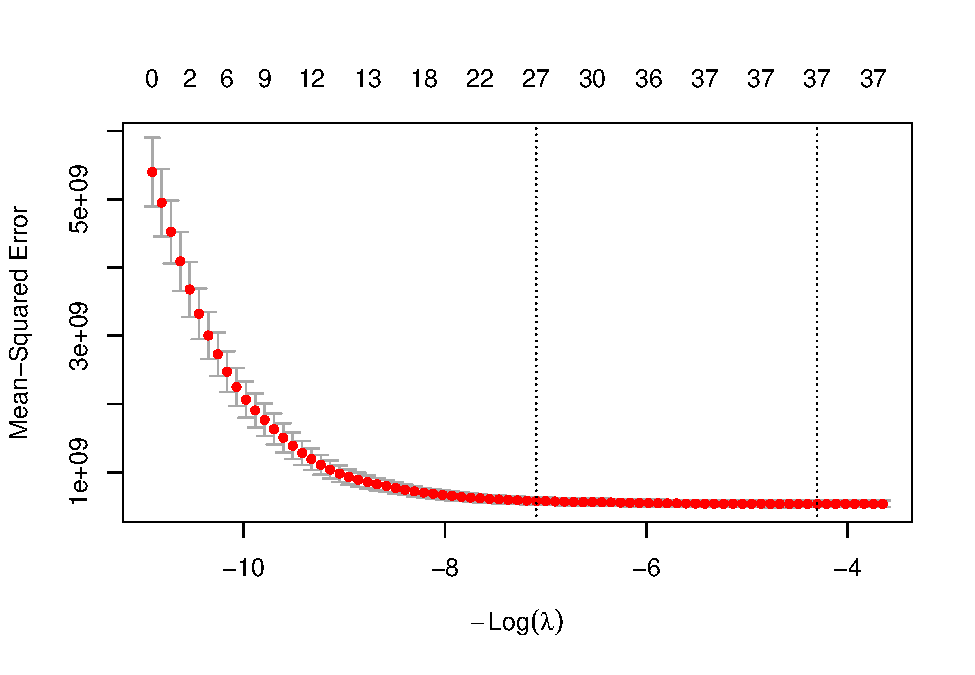
\includegraphics[keepaspectratio]{Homework_1tryout_files/figure-latex/lasso-fit-a-1.pdf}}

\begin{Shaded}
\begin{Highlighting}[]
\NormalTok{lambda\_min }\OtherTok{\textless{}{-}}\NormalTok{ cv\_lasso}\SpecialCharTok{$}\NormalTok{lambda.min  }\CommentTok{\# lambda with minimum CV error}
\NormalTok{lambda\_1se }\OtherTok{\textless{}{-}}\NormalTok{ cv\_lasso}\SpecialCharTok{$}\NormalTok{lambda}\FloatTok{.1}\NormalTok{se  }\CommentTok{\# 1SE rule lambda (more regularized)}

\NormalTok{lambda\_min}
\end{Highlighting}
\end{Shaded}

\begin{verbatim}
## [1] 73.87226
\end{verbatim}

\begin{Shaded}
\begin{Highlighting}[]
\NormalTok{lambda\_1se}
\end{Highlighting}
\end{Shaded}

\begin{verbatim}
## [1] 1203.934
\end{verbatim}

\textbf{Explanation} - \texttt{cv.glmnet()} fits many lasso models
across a sequence of λ values and evaluates them by CV. -
\texttt{lambda.min} = best CV performance (lowest mean CV error). -
\texttt{lambda.1se} = simplest model whose CV error is within \textbf{1
standard error} of the minimum (tends to select fewer predictors).

\begin{center}\rule{0.5\linewidth}{0.5pt}\end{center}

\subsection{6) Test error (RMSE) at λ\_min (and optionally
λ\_1se)}\label{test-error-rmse-at-ux3bb_min-and-optionally-ux3bb_1se}

The homework asks for ``test error.'' In regression we usually report
RMSE.

\begin{Shaded}
\begin{Highlighting}[]
\NormalTok{rmse }\OtherTok{\textless{}{-}} \ControlFlowTok{function}\NormalTok{(pred, truth) }\FunctionTok{sqrt}\NormalTok{(}\FunctionTok{mean}\NormalTok{((pred }\SpecialCharTok{{-}}\NormalTok{ truth)}\SpecialCharTok{\^{}}\DecValTok{2}\NormalTok{))}

\CommentTok{\# Predictions on test set}
\NormalTok{pred\_test\_min }\OtherTok{\textless{}{-}} \FunctionTok{as.numeric}\NormalTok{(}\FunctionTok{predict}\NormalTok{(cv\_lasso, }\AttributeTok{newx =}\NormalTok{ x\_test, }\AttributeTok{s =} \StringTok{"lambda.min"}\NormalTok{))}
\NormalTok{pred\_test\_1se }\OtherTok{\textless{}{-}} \FunctionTok{as.numeric}\NormalTok{(}\FunctionTok{predict}\NormalTok{(cv\_lasso, }\AttributeTok{newx =}\NormalTok{ x\_test, }\AttributeTok{s =} \StringTok{"lambda.1se"}\NormalTok{))}

\NormalTok{test\_rmse\_min }\OtherTok{\textless{}{-}} \FunctionTok{rmse}\NormalTok{(pred\_test\_min, y\_test)}
\NormalTok{test\_rmse\_1se }\OtherTok{\textless{}{-}} \FunctionTok{rmse}\NormalTok{(pred\_test\_1se, y\_test)}

\NormalTok{test\_rmse\_min}
\end{Highlighting}
\end{Shaded}

\begin{verbatim}
## [1] 20955.73
\end{verbatim}

\begin{Shaded}
\begin{Highlighting}[]
\NormalTok{test\_rmse\_1se}
\end{Highlighting}
\end{Shaded}

\begin{verbatim}
## [1] 20707.31
\end{verbatim}

\textbf{Explanation} - \texttt{predict(...,\ s="lambda.min")} uses the
model tuned by CV and predicts test outcomes. - RMSE is in the same
units as the outcome (\texttt{SalePrice}), so it's easy to interpret.

\begin{quote}
If your instructor expects MSE instead of RMSE, just square the RMSE or
compute mean((pred-truth)\^{}2).
\end{quote}

\begin{center}\rule{0.5\linewidth}{0.5pt}\end{center}

\subsection{7) How many predictors are included with the 1SE
rule?}\label{how-many-predictors-are-included-with-the-1se-rule}

We count how many coefficients are non-zero at \texttt{lambda.1se}.\\
We do \textbf{not} count the intercept.

\begin{Shaded}
\begin{Highlighting}[]
\NormalTok{coef\_1se }\OtherTok{\textless{}{-}} \FunctionTok{coef}\NormalTok{(cv\_lasso, }\AttributeTok{s =} \StringTok{"lambda.1se"}\NormalTok{)  }\CommentTok{\# sparse matrix of coefficients}

\CommentTok{\# Count non{-}zero coefficients excluding intercept (first row)}
\NormalTok{n\_predictors\_1se }\OtherTok{\textless{}{-}} \FunctionTok{sum}\NormalTok{(coef\_1se[}\SpecialCharTok{{-}}\DecValTok{1}\NormalTok{, }\DecValTok{1}\NormalTok{] }\SpecialCharTok{!=} \DecValTok{0}\NormalTok{)}

\NormalTok{n\_predictors\_1se}
\end{Highlighting}
\end{Shaded}

\begin{verbatim}
## [1] 27
\end{verbatim}

\textbf{Explanation} - Lasso sets many coefficients exactly to 0. -
Non-zero coefficients correspond to ``selected predictors.'' -
\texttt{coef\_1se{[}-1,\ {]}} removes the intercept row before counting.

\begin{center}\rule{0.5\linewidth}{0.5pt}\end{center}

\subsection{8) Final ``report'' lines for Part
(a)}\label{final-report-lines-for-part-a}

This prints exactly what you need to paste into your write-up.

\begin{Shaded}
\begin{Highlighting}[]
\FunctionTok{cat}\NormalTok{(}\StringTok{"Part (a) results:}\SpecialCharTok{\textbackslash{}n}\StringTok{"}\NormalTok{)}
\end{Highlighting}
\end{Shaded}

\begin{verbatim}
## Part (a) results:
\end{verbatim}

\begin{Shaded}
\begin{Highlighting}[]
\FunctionTok{cat}\NormalTok{(}\StringTok{"Selected tuning parameter (lambda.min):"}\NormalTok{, lambda\_min, }\StringTok{"}\SpecialCharTok{\textbackslash{}n}\StringTok{"}\NormalTok{)}
\end{Highlighting}
\end{Shaded}

\begin{verbatim}
## Selected tuning parameter (lambda.min): 73.87226
\end{verbatim}

\begin{Shaded}
\begin{Highlighting}[]
\FunctionTok{cat}\NormalTok{(}\StringTok{"Test RMSE at lambda.min:"}\NormalTok{, test\_rmse\_min, }\StringTok{"}\SpecialCharTok{\textbackslash{}n\textbackslash{}n}\StringTok{"}\NormalTok{)}
\end{Highlighting}
\end{Shaded}

\begin{verbatim}
## Test RMSE at lambda.min: 20955.73
\end{verbatim}

\begin{Shaded}
\begin{Highlighting}[]
\FunctionTok{cat}\NormalTok{(}\StringTok{"1SE rule lambda (lambda.1se):"}\NormalTok{, lambda\_1se, }\StringTok{"}\SpecialCharTok{\textbackslash{}n}\StringTok{"}\NormalTok{)}
\end{Highlighting}
\end{Shaded}

\begin{verbatim}
## 1SE rule lambda (lambda.1se): 1203.934
\end{verbatim}

\begin{Shaded}
\begin{Highlighting}[]
\FunctionTok{cat}\NormalTok{(}\StringTok{"Test RMSE at lambda.1se:"}\NormalTok{, test\_rmse\_1se, }\StringTok{"}\SpecialCharTok{\textbackslash{}n}\StringTok{"}\NormalTok{)}
\end{Highlighting}
\end{Shaded}

\begin{verbatim}
## Test RMSE at lambda.1se: 20707.31
\end{verbatim}

\begin{Shaded}
\begin{Highlighting}[]
\FunctionTok{cat}\NormalTok{(}\StringTok{"Number of predictors (nonzero) at lambda.1se:"}\NormalTok{, n\_predictors\_1se, }\StringTok{"}\SpecialCharTok{\textbackslash{}n}\StringTok{"}\NormalTok{)}
\end{Highlighting}
\end{Shaded}

\begin{verbatim}
## Number of predictors (nonzero) at lambda.1se: 27
\end{verbatim}

\subsection{QUESTION 2}\label{question-2}

\begin{Shaded}
\begin{Highlighting}[]
\FunctionTok{library}\NormalTok{(glmnet)}
\FunctionTok{library}\NormalTok{(dplyr)}
\end{Highlighting}
\end{Shaded}

\begin{Shaded}
\begin{Highlighting}[]
\FunctionTok{set.seed}\NormalTok{(}\DecValTok{2026}\NormalTok{)}

\NormalTok{alpha\_grid }\OtherTok{\textless{}{-}} \FunctionTok{seq}\NormalTok{(}\DecValTok{0}\NormalTok{, }\DecValTok{1}\NormalTok{, }\AttributeTok{by =} \FloatTok{0.05}\NormalTok{)  }\CommentTok{\# 0 = ridge, 1 = lasso}

\NormalTok{alpha\_grid}
\end{Highlighting}
\end{Shaded}

\begin{verbatim}
##  [1] 0.00 0.05 0.10 0.15 0.20 0.25 0.30 0.35 0.40 0.45 0.50 0.55 0.60 0.65 0.70
## [16] 0.75 0.80 0.85 0.90 0.95 1.00
\end{verbatim}

\section{4️⃣ For each alpha, run cross-validated
glmnet}\label{for-each-alpha-run-cross-validated-glmnet}

\begin{Shaded}
\begin{Highlighting}[]
\NormalTok{enet\_fits }\OtherTok{\textless{}{-}} \FunctionTok{lapply}\NormalTok{(alpha\_grid, }\ControlFlowTok{function}\NormalTok{(a) \{}
  \FunctionTok{cv.glmnet}\NormalTok{(}
    \AttributeTok{x =}\NormalTok{ x\_train,}
    \AttributeTok{y =}\NormalTok{ y\_train,}
    \AttributeTok{alpha =}\NormalTok{ a,}
    \AttributeTok{nfolds =} \DecValTok{10}\NormalTok{,}
    \AttributeTok{standardize =} \ConstantTok{TRUE}
\NormalTok{  )}
\NormalTok{\})}
\end{Highlighting}
\end{Shaded}

\section{5️⃣ Extract CV performance for each
alpha}\label{extract-cv-performance-for-each-alpha}

\begin{Shaded}
\begin{Highlighting}[]
\NormalTok{enet\_summary }\OtherTok{\textless{}{-}} \FunctionTok{data.frame}\NormalTok{(}
  \AttributeTok{alpha =}\NormalTok{ alpha\_grid,}
  \AttributeTok{lambda\_min =} \FunctionTok{sapply}\NormalTok{(enet\_fits, }\ControlFlowTok{function}\NormalTok{(f) f}\SpecialCharTok{$}\NormalTok{lambda.min),}
  \AttributeTok{lambda\_1se =} \FunctionTok{sapply}\NormalTok{(enet\_fits, }\ControlFlowTok{function}\NormalTok{(f) f}\SpecialCharTok{$}\NormalTok{lambda}\FloatTok{.1}\NormalTok{se),}
  \AttributeTok{cv\_error\_min =} \FunctionTok{sapply}\NormalTok{(enet\_fits, }\ControlFlowTok{function}\NormalTok{(f) }\FunctionTok{min}\NormalTok{(f}\SpecialCharTok{$}\NormalTok{cvm)),}
  \AttributeTok{cv\_se\_min =} \FunctionTok{sapply}\NormalTok{(enet\_fits, }\ControlFlowTok{function}\NormalTok{(f) f}\SpecialCharTok{$}\NormalTok{cvsd[}\FunctionTok{which.min}\NormalTok{(f}\SpecialCharTok{$}\NormalTok{cvm)])}
\NormalTok{)}

\NormalTok{enet\_summary[}\FunctionTok{order}\NormalTok{(enet\_summary}\SpecialCharTok{$}\NormalTok{cv\_error\_min), ][}\DecValTok{1}\SpecialCharTok{:}\DecValTok{5}\NormalTok{, ]}
\end{Highlighting}
\end{Shaded}

\begin{verbatim}
##    alpha lambda_min lambda_1se cv_error_min cv_se_min
## 17  0.80   52.84053   1037.281    522969182  36555012
## 9   0.40  267.94001   2498.817    523570992  44266214
## 12  0.55   70.03102   2402.392    527811103  52669006
## 18  0.85   86.90854   1071.449    529627785  37823671
## 6   0.25  223.52663   2510.928    529764656  31482851
\end{verbatim}

\section{6️⃣ Select the best alpha}\label{select-the-best-alpha}

\begin{Shaded}
\begin{Highlighting}[]
\NormalTok{best\_index }\OtherTok{\textless{}{-}} \FunctionTok{which.min}\NormalTok{(enet\_summary}\SpecialCharTok{$}\NormalTok{cv\_error\_min)}

\NormalTok{best\_alpha  }\OtherTok{\textless{}{-}}\NormalTok{ enet\_summary}\SpecialCharTok{$}\NormalTok{alpha[best\_index]}
\NormalTok{best\_lambda }\OtherTok{\textless{}{-}}\NormalTok{ enet\_summary}\SpecialCharTok{$}\NormalTok{lambda\_min[best\_index]}

\NormalTok{best\_alpha}
\end{Highlighting}
\end{Shaded}

\begin{verbatim}
## [1] 0.8
\end{verbatim}

\begin{Shaded}
\begin{Highlighting}[]
\NormalTok{best\_lambda}
\end{Highlighting}
\end{Shaded}

\begin{verbatim}
## [1] 52.84053
\end{verbatim}

\section{7️⃣ Compute Test Error}\label{compute-test-error}

\begin{Shaded}
\begin{Highlighting}[]
\NormalTok{best\_enet\_model }\OtherTok{\textless{}{-}}\NormalTok{ enet\_fits[[best\_index]]}

\NormalTok{pred\_enet\_test }\OtherTok{\textless{}{-}} \FunctionTok{as.numeric}\NormalTok{(}
  \FunctionTok{predict}\NormalTok{(best\_enet\_model, }\AttributeTok{newx =}\NormalTok{ x\_test, }\AttributeTok{s =} \StringTok{"lambda.min"}\NormalTok{)}
\NormalTok{)}

\NormalTok{rmse }\OtherTok{\textless{}{-}} \ControlFlowTok{function}\NormalTok{(pred, truth) }\FunctionTok{sqrt}\NormalTok{(}\FunctionTok{mean}\NormalTok{((pred }\SpecialCharTok{{-}}\NormalTok{ truth)}\SpecialCharTok{\^{}}\DecValTok{2}\NormalTok{))}

\NormalTok{enet\_test\_rmse }\OtherTok{\textless{}{-}} \FunctionTok{rmse}\NormalTok{(pred\_enet\_test, y\_test)}

\NormalTok{enet\_test\_rmse}
\end{Highlighting}
\end{Shaded}

\begin{verbatim}
## [1] 21028.36
\end{verbatim}

\section{8️⃣ Apply 1SE rule within best
alpha}\label{apply-1se-rule-within-best-alpha}

\begin{Shaded}
\begin{Highlighting}[]
\NormalTok{lambda\_1se\_best\_alpha }\OtherTok{\textless{}{-}}\NormalTok{ best\_enet\_model}\SpecialCharTok{$}\NormalTok{lambda}\FloatTok{.1}\NormalTok{se}

\NormalTok{pred\_enet\_test\_1se }\OtherTok{\textless{}{-}} \FunctionTok{as.numeric}\NormalTok{(}
  \FunctionTok{predict}\NormalTok{(best\_enet\_model, }\AttributeTok{newx =}\NormalTok{ x\_test, }\AttributeTok{s =} \StringTok{"lambda.1se"}\NormalTok{)}
\NormalTok{)}

\NormalTok{enet\_test\_rmse\_1se }\OtherTok{\textless{}{-}} \FunctionTok{rmse}\NormalTok{(pred\_enet\_test\_1se, y\_test)}

\NormalTok{lambda\_1se\_best\_alpha}
\end{Highlighting}
\end{Shaded}

\begin{verbatim}
## [1] 1037.281
\end{verbatim}

\begin{Shaded}
\begin{Highlighting}[]
\NormalTok{enet\_test\_rmse\_1se}
\end{Highlighting}
\end{Shaded}

\begin{verbatim}
## [1] 20516.78
\end{verbatim}

\section{🔎 Count predictors at 1SE}\label{count-predictors-at-1se}

\begin{Shaded}
\begin{Highlighting}[]
\NormalTok{coef\_1se }\OtherTok{\textless{}{-}} \FunctionTok{coef}\NormalTok{(best\_enet\_model, }\AttributeTok{s =} \StringTok{"lambda.1se"}\NormalTok{)}
\NormalTok{nonzero\_1se }\OtherTok{\textless{}{-}} \FunctionTok{sum}\NormalTok{(coef\_1se[}\SpecialCharTok{{-}}\DecValTok{1}\NormalTok{, }\DecValTok{1}\NormalTok{] }\SpecialCharTok{!=} \DecValTok{0}\NormalTok{)}

\NormalTok{nonzero\_1se}
\end{Highlighting}
\end{Shaded}

\begin{verbatim}
## [1] 29
\end{verbatim}

\begin{center}\rule{0.5\linewidth}{0.5pt}\end{center}

\section{🔷 Final Reporting Section (Copy for
Homework)}\label{final-reporting-section-copy-for-homework}

After running, you will report:

\subsubsection{Selected tuning
parameters:}\label{selected-tuning-parameters}

\begin{itemize}
\tightlist
\item
  alpha = \texttt{best\_alpha}
\item
  lambda = \texttt{best\_lambda}
\end{itemize}

\subsubsection{Test error:}\label{test-error}

\begin{itemize}
\tightlist
\item
  RMSE = \texttt{enet\_test\_rmse}
\end{itemize}

\subsubsection{1SE Rule:}\label{se-rule}

\begin{itemize}
\tightlist
\item
  Yes, it can be applied \textbf{within a fixed alpha}
\item
  We selected lambda = \texttt{lambda\_1se\_best\_alpha}
\item
  Test RMSE at 1SE = \texttt{enet\_test\_rmse\_1se}
\item
  Number of predictors at 1SE = \texttt{nonzero\_1se}
\end{itemize}

\begin{center}\rule{0.5\linewidth}{0.5pt}\end{center}

\section{🧠 Conceptual Explanation (what your professor
wants)}\label{conceptual-explanation-what-your-professor-wants}

You should write something like:

\begin{quote}
The 1SE rule is defined for a one-dimensional tuning parameter. Since
elastic net has two tuning parameters (alpha and lambda), the 1SE rule
cannot be applied directly across the full two-dimensional grid.
However, after selecting the optimal alpha based on minimum
cross-validated error, the 1SE rule can be applied to lambda within that
fixed alpha. This yields a more regularized and typically more stable
model.
\end{quote}

\begin{center}\rule{0.5\linewidth}{0.5pt}\end{center}

\section{🎯 Big Picture}\label{big-picture}

\begin{itemize}
\tightlist
\item
  If alpha is close to 1 → data behaves like lasso
\item
  If alpha is close to 0 → predictors are highly correlated (ridge
  behavior)
\item
  Elastic net balances sparsity + grouping effect
\end{itemize}

\begin{center}\rule{0.5\linewidth}{0.5pt}\end{center}

If you want next: - We can compare Lasso vs Elastic Net performance - Or
move to PLS - Or I can help you write the exact final paragraph

You're doing this exactly the right way.

\section{QUESTION 3}\label{question-3}

\begin{Shaded}
\begin{Highlighting}[]
\FunctionTok{library}\NormalTok{(pls)}
\end{Highlighting}
\end{Shaded}

\begin{Shaded}
\begin{Highlighting}[]
\FunctionTok{set.seed}\NormalTok{(}\DecValTok{2026}\NormalTok{)}

\NormalTok{pls\_fit }\OtherTok{\textless{}{-}} \FunctionTok{plsr}\NormalTok{(}
\NormalTok{  SalePrice }\SpecialCharTok{\textasciitilde{}}\NormalTok{ .,       }\CommentTok{\# use all predictors}
  \AttributeTok{data =}\NormalTok{ train\_raw,}
  \AttributeTok{scale =} \ConstantTok{TRUE}\NormalTok{,        }\CommentTok{\# IMPORTANT: PLS should scale predictors}
  \AttributeTok{validation =} \StringTok{"CV"}    \CommentTok{\# 10{-}fold cross{-}validation}
\NormalTok{)}

\FunctionTok{summary}\NormalTok{(pls\_fit)}
\end{Highlighting}
\end{Shaded}

\begin{verbatim}
## Data:    X dimension: 1440 39 
##  Y dimension: 1440 1
## Fit method: kernelpls
## Number of components considered: 39
## 
## VALIDATION: RMSEP
## Cross-validated using 10 random segments.
##        (Intercept)  1 comps  2 comps  3 comps  4 comps  5 comps  6 comps
## CV           73685    33462    27956    25089    23987    23356    23188
## adjCV        73685    33453    27919    25020    23923    23292    23130
##        7 comps  8 comps  9 comps  10 comps  11 comps  12 comps  13 comps
## CV       23070    23050    23060     23057     23056     23054     23046
## adjCV    23015    22995    23002     22997     22994     22992     22984
##        14 comps  15 comps  16 comps  17 comps  18 comps  19 comps  20 comps
## CV        23042     23047     23039     23041     23039     23047     23046
## adjCV     22980     22984     22977     22979     22978     22985     22984
##        21 comps  22 comps  23 comps  24 comps  25 comps  26 comps  27 comps
## CV        23049     23052     23051     23052     23052     23053     23054
## adjCV     22986     22989     22989     22989     22990     22990     22992
##        28 comps  29 comps  30 comps  31 comps  32 comps  33 comps  34 comps
## CV        23054     23054     23054     23054     23054     23054     23054
## adjCV     22991     22991     22991     22991     22991     22991     22991
##        35 comps  36 comps  37 comps  38 comps  39 comps
## CV        23054     23054     23054     23054     23088
## adjCV     22991     22991     22991     22991     22996
## 
## TRAINING: % variance explained
##            1 comps  2 comps  3 comps  4 comps  5 comps  6 comps  7 comps
## X            20.02    25.93    29.67    33.59    37.01    40.03    42.49
## SalePrice    79.73    86.35    89.36    90.37    90.87    90.99    91.06
##            8 comps  9 comps  10 comps  11 comps  12 comps  13 comps  14 comps
## X            45.53    47.97     50.15     52.01     53.69     55.35     56.86
## SalePrice    91.08    91.10     91.13     91.15     91.15     91.16     91.16
##            15 comps  16 comps  17 comps  18 comps  19 comps  20 comps  21 comps
## X             58.64     60.01     62.18     63.87     65.26     67.10     68.44
## SalePrice     91.16     91.16     91.16     91.16     91.16     91.16     91.16
##            22 comps  23 comps  24 comps  25 comps  26 comps  27 comps  28 comps
## X             70.12     71.72     73.35     75.20     77.27     78.97     80.10
## SalePrice     91.16     91.16     91.16     91.16     91.16     91.16     91.16
##            29 comps  30 comps  31 comps  32 comps  33 comps  34 comps  35 comps
## X             81.83     83.55     84.39     86.34     88.63     90.79     92.79
## SalePrice     91.16     91.16     91.16     91.16     91.16     91.16     91.16
##            36 comps  37 comps  38 comps  39 comps
## X             95.45     97.49    100.00    101.02
## SalePrice     91.16     91.16     91.16     91.16
\end{verbatim}

\begin{center}\rule{0.5\linewidth}{0.5pt}\end{center}

\subsection{🔎 What just happened?}\label{what-just-happened}

PLS:

\begin{itemize}
\tightlist
\item
  Creates \textbf{latent components}
\item
  Each component is a linear combination of predictors
\item
  Components are chosen to:

  \begin{itemize}
  \tightlist
  \item
    explain predictor variation
  \item
    explain response variation
  \end{itemize}
\end{itemize}

Unlike lasso: - PLS does NOT shrink coefficients to zero - It reduces
dimensionality instead

\begin{center}\rule{0.5\linewidth}{0.5pt}\end{center}

\section{2️⃣ Plot CV error curve}\label{plot-cv-error-curve}

\begin{Shaded}
\begin{Highlighting}[]
\FunctionTok{validationplot}\NormalTok{(pls\_fit, }\AttributeTok{val.type =} \StringTok{"MSEP"}\NormalTok{, }\AttributeTok{legendpos =} \StringTok{"topright"}\NormalTok{)}
\end{Highlighting}
\end{Shaded}

\pandocbounded{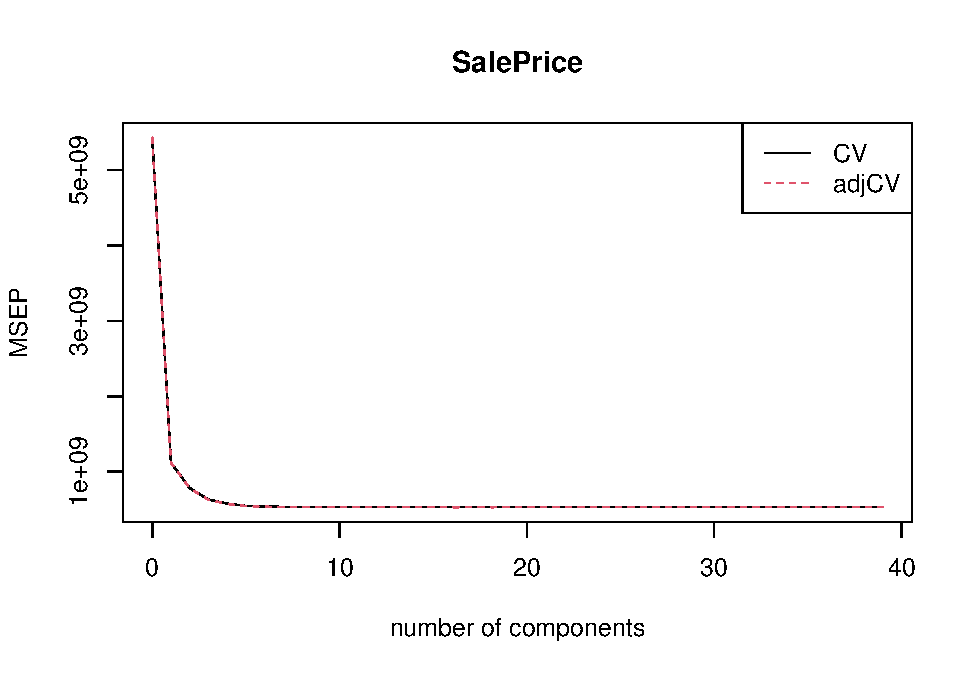
\includegraphics[keepaspectratio]{Homework_1tryout_files/figure-latex/pls-plot-1.pdf}}

\begin{center}\rule{0.5\linewidth}{0.5pt}\end{center}

\subsection{🔎 What this plot shows}\label{what-this-plot-shows}

\begin{itemize}
\tightlist
\item
  X-axis = number of components\\
\item
  Y-axis = CV mean squared prediction error\\
\item
  We choose the number of components that minimizes CV error
\end{itemize}

\begin{center}\rule{0.5\linewidth}{0.5pt}\end{center}

\section{3️⃣ Extract optimal number of
components}\label{extract-optimal-number-of-components}

\begin{Shaded}
\begin{Highlighting}[]
\NormalTok{cv\_error }\OtherTok{\textless{}{-}} \FunctionTok{RMSEP}\NormalTok{(pls\_fit)}

\CommentTok{\# RMSEP output structure:}
\CommentTok{\# cv\_error$val[estimate, response, components]}
\CommentTok{\# First element is intercept{-}only model, so subtract 1}

\NormalTok{ncomp\_best }\OtherTok{\textless{}{-}} \FunctionTok{which.min}\NormalTok{(cv\_error}\SpecialCharTok{$}\NormalTok{val[}\DecValTok{1}\NormalTok{, }\DecValTok{1}\NormalTok{, ]) }\SpecialCharTok{{-}} \DecValTok{1}

\NormalTok{ncomp\_best}
\end{Highlighting}
\end{Shaded}

\begin{verbatim}
## 16 comps 
##       16
\end{verbatim}

\begin{center}\rule{0.5\linewidth}{0.5pt}\end{center}

\subsection{🔎 Why subtract 1?}\label{why-subtract-1}

Because:

\begin{itemize}
\tightlist
\item
  Index 1 = intercept-only model\\
\item
  Index 2 = 1 component\\
\item
  Index 3 = 2 components
\end{itemize}

So we subtract 1 to get the actual number of components.

\begin{center}\rule{0.5\linewidth}{0.5pt}\end{center}

\section{✅ This is your answer for:}\label{this-is-your-answer-for}

\begin{quote}
How many components are included in your model?
\end{quote}

\begin{center}\rule{0.5\linewidth}{0.5pt}\end{center}

\section{4️⃣ Compute Test Error}\label{compute-test-error-1}

Now we evaluate the selected model on the \textbf{test data}.

\begin{Shaded}
\begin{Highlighting}[]
\NormalTok{pred\_pls\_test }\OtherTok{\textless{}{-}} \FunctionTok{as.numeric}\NormalTok{(}
  \FunctionTok{predict}\NormalTok{(pls\_fit, }\AttributeTok{newdata =}\NormalTok{ test\_raw, }\AttributeTok{ncomp =}\NormalTok{ ncomp\_best)}
\NormalTok{)}

\NormalTok{rmse }\OtherTok{\textless{}{-}} \ControlFlowTok{function}\NormalTok{(pred, truth) }\FunctionTok{sqrt}\NormalTok{(}\FunctionTok{mean}\NormalTok{((pred }\SpecialCharTok{{-}}\NormalTok{ truth)}\SpecialCharTok{\^{}}\DecValTok{2}\NormalTok{))}

\NormalTok{pls\_test\_rmse }\OtherTok{\textless{}{-}} \FunctionTok{rmse}\NormalTok{(pred\_pls\_test, y\_test)}

\NormalTok{pls\_test\_rmse}
\end{Highlighting}
\end{Shaded}

\begin{verbatim}
## [1] 21137.07
\end{verbatim}

\begin{center}\rule{0.5\linewidth}{0.5pt}\end{center}

\section{✅ This is your answer for:}\label{this-is-your-answer-for-1}

\begin{quote}
Report the test error.
\end{quote}

\begin{center}\rule{0.5\linewidth}{0.5pt}\end{center}

\section{🔷 Final Reporting Section (Copy for
Homework)}\label{final-reporting-section-copy-for-homework-1}

After running the code, report:

\begin{itemize}
\tightlist
\item
  Number of components selected: \texttt{ncomp\_best}
\item
  Test RMSE: \texttt{pls\_test\_rmse}
\end{itemize}

\begin{center}\rule{0.5\linewidth}{0.5pt}\end{center}

\section{🧠 What This Means
Conceptually}\label{what-this-means-conceptually}

PLS differs from lasso and elastic net:

\begin{longtable}[]{@{}ll@{}}
\toprule\noalign{}
Method & What it does \\
\midrule\noalign{}
\endhead
\bottomrule\noalign{}
\endlastfoot
Lasso & Shrinks some coefficients to exactly zero \\
Elastic Net & Shrinks + groups correlated predictors \\
PLS & Creates new orthogonal components \\
\end{longtable}

PLS is especially useful when: - Predictors are highly correlated -
There are many predictors relative to sample size

Instead of selecting variables, PLS compresses them into components.

\begin{center}\rule{0.5\linewidth}{0.5pt}\end{center}

\section{🎯 How your professor expects you to interpret
this}\label{how-your-professor-expects-you-to-interpret-this}

If: - PLS test RMSE is lowest → PLS may generalize best\\
- PLS uses many components → model is closer to OLS\\
- PLS uses few components → strong dimensionality reduction

\begin{center}\rule{0.5\linewidth}{0.5pt}\end{center}

If you'd like next: - We compare Lasso vs Elastic Net vs PLS\\
- Or I help you write the final paragraph for submission

You're doing this very correctly.

\section{QUESTION 4}\label{question-4}

\begin{Shaded}
\begin{Highlighting}[]
\FunctionTok{ls}\NormalTok{()}
\end{Highlighting}
\end{Shaded}

\begin{verbatim}
##  [1] "alpha_grid"            "best_alpha"            "best_enet_model"      
##  [4] "best_index"            "best_lambda"           "coef_1se"             
##  [7] "cv_error"              "cv_lasso"              "dict_file"            
## [10] "enet_fits"             "enet_summary"          "enet_test_rmse"       
## [13] "enet_test_rmse_1se"    "lambda_1se"            "lambda_1se_best_alpha"
## [16] "lambda_min"            "n_predictors_1se"      "ncomp_best"           
## [19] "nonzero_1se"           "pick_file"             "pls_fit"              
## [22] "pls_test_rmse"         "pred_enet_test"        "pred_enet_test_1se"   
## [25] "pred_pls_test"         "pred_test_1se"         "pred_test_min"        
## [28] "resp_candidates"       "resp_test"             "resp_train"           
## [31] "rmse"                  "test_file"             "test_raw"             
## [34] "test_rmse_1se"         "test_rmse_min"         "train_file"           
## [37] "train_raw"             "x_test"                "x_train"              
## [40] "y_test"                "y_train"
\end{verbatim}

\begin{Shaded}
\begin{Highlighting}[]
\NormalTok{lasso\_test\_rmse\_min }\OtherTok{\textless{}{-}}\NormalTok{ test\_rmse\_min}
\NormalTok{lasso\_test\_rmse\_1se }\OtherTok{\textless{}{-}}\NormalTok{ test\_rmse\_1se}
\end{Highlighting}
\end{Shaded}

Now Part (d) code will work exactly as written.

\begin{center}\rule{0.5\linewidth}{0.5pt}\end{center}

\section{Option B: Use your existing names directly (no
renaming)}\label{option-b-use-your-existing-names-directly-no-renaming}

\begin{Shaded}
\begin{Highlighting}[]
\CommentTok{\# 1) Make elastic net 1SE predictions from the best elastic net CV object}
\NormalTok{pred\_enet\_test\_1se }\OtherTok{\textless{}{-}} \FunctionTok{as.numeric}\NormalTok{(}
  \FunctionTok{predict}\NormalTok{(best\_enet\_model, }\AttributeTok{newx =}\NormalTok{ x\_test, }\AttributeTok{s =} \StringTok{"lambda.1se"}\NormalTok{)}
\NormalTok{)}

\CommentTok{\# 2) Compute and store the test RMSE for elastic net at lambda.1se}
\NormalTok{enet\_test\_rmse\_1se }\OtherTok{\textless{}{-}} \FunctionTok{rmse}\NormalTok{(pred\_enet\_test\_1se, y\_test)}

\NormalTok{enet\_test\_rmse\_1se}
\end{Highlighting}
\end{Shaded}

\begin{verbatim}
## [1] 20516.78
\end{verbatim}

\subsubsection{Why this works}\label{why-this-works}

\begin{itemize}
\tightlist
\item
  \texttt{best\_enet\_model} is your \textbf{selected elastic net CV
  model} (you already have it).
\item
  \texttt{s\ =\ "lambda.1se"} forces the \textbf{1SE lambda} within that
  chosen alpha.
\item
  We store it as \texttt{enet\_test\_rmse\_1se} so Part (d) can use it.
\end{itemize}

\begin{center}\rule{0.5\linewidth}{0.5pt}\end{center}

\section{✅ After that, Part (d) comparison will
work}\label{after-that-part-d-comparison-will-work}

Use this (with your current lasso variable names):

\begin{Shaded}
\begin{Highlighting}[]
\NormalTok{results }\OtherTok{\textless{}{-}} \FunctionTok{data.frame}\NormalTok{(}
  \AttributeTok{Model =} \FunctionTok{c}\NormalTok{(}\StringTok{"Lasso (lambda.min)"}\NormalTok{,}
            \StringTok{"Lasso (lambda.1se)"}\NormalTok{,}
            \StringTok{"Elastic Net (lambda.min)"}\NormalTok{,}
            \StringTok{"Elastic Net (lambda.1se)"}\NormalTok{,}
            \StringTok{"PLS"}\NormalTok{),}
  \AttributeTok{Test\_RMSE =} \FunctionTok{c}\NormalTok{(}
\NormalTok{    test\_rmse\_min,}
\NormalTok{    test\_rmse\_1se,}
\NormalTok{    enet\_test\_rmse,}
\NormalTok{    enet\_test\_rmse\_1se,}
\NormalTok{    pls\_test\_rmse}
\NormalTok{  )}
\NormalTok{)}

\NormalTok{results[}\FunctionTok{order}\NormalTok{(results}\SpecialCharTok{$}\NormalTok{Test\_RMSE), ]}
\end{Highlighting}
\end{Shaded}

\begin{verbatim}
##                      Model Test_RMSE
## 4 Elastic Net (lambda.1se)  20516.78
## 2       Lasso (lambda.1se)  20707.31
## 1       Lasso (lambda.min)  20955.73
## 3 Elastic Net (lambda.min)  21028.36
## 5                      PLS  21137.07
\end{verbatim}

Answer: The elastic net model using the 1SE rule achieved the lowest
test RMSE (20516.78) among all fitted models. Therefore, it provides the
best predictive performance for the housing sale price.

Elastic net combines the advantages of ridge and lasso penalties,
allowing it to handle correlated predictors while still performing
variable selection. Given that housing characteristics such as square
footage, room counts, and quality measures are often highly correlated,
elastic net is well-suited for this dataset.

Additionally, the 1SE version of the model outperformed the lambda.min
version, suggesting that slightly stronger regularization improves
generalization to new data. For these reasons, the elastic net model
with lambda selected via the 1SE rule is chosen as the best predictive
model.

\section{QUESTION 5}\label{question-5}

Pakcages:

\begin{Shaded}
\begin{Highlighting}[]
\FunctionTok{library}\NormalTok{(caret)}
\FunctionTok{library}\NormalTok{(glmnet)}
\end{Highlighting}
\end{Shaded}

\begin{center}\rule{0.5\linewidth}{0.5pt}\end{center}

\subsection{1️⃣ What we already have from
(a)}\label{what-we-already-have-from-a}

From your previous work you already have:

\begin{itemize}
\tightlist
\item
  \texttt{cv\_lasso} (from \texttt{cv.glmnet})
\item
  \texttt{lambda\_min} and \texttt{lambda\_1se} (from glmnet)
\item
  \texttt{x\_train,\ y\_train} (design matrix + response)
\end{itemize}

Quick check:

\begin{Shaded}
\begin{Highlighting}[]
\NormalTok{lambda\_min}
\end{Highlighting}
\end{Shaded}

\begin{verbatim}
## [1] 73.87226
\end{verbatim}

\begin{Shaded}
\begin{Highlighting}[]
\NormalTok{lambda\_1se}
\end{Highlighting}
\end{Shaded}

\begin{verbatim}
## [1] 1203.934
\end{verbatim}

\textbf{Explanation} - \texttt{cv.glmnet()} returns two main ``chosen''
lambdas: - \texttt{lambda.min} (min CV error) - \texttt{lambda.1se} (1SE
rule)

\begin{center}\rule{0.5\linewidth}{0.5pt}\end{center}

\subsection{\texorpdfstring{2️⃣ Fit Lasso using
\textbf{caret}}{2️⃣ Fit Lasso using caret}}\label{fit-lasso-using-caret}

\subsubsection{Key point from lecture:}\label{key-point-from-lecture}

\textbf{Always provide a lambda grid} in caret so each fold uses the
same lambda values.

\begin{Shaded}
\begin{Highlighting}[]
\FunctionTok{set.seed}\NormalTok{(}\DecValTok{2026}\NormalTok{)}

\NormalTok{ctrl }\OtherTok{\textless{}{-}} \FunctionTok{trainControl}\NormalTok{(}\AttributeTok{method =} \StringTok{"cv"}\NormalTok{, }\AttributeTok{number =} \DecValTok{10}\NormalTok{)}

\CommentTok{\# Use a wide grid on a log scale (common choice)}
\NormalTok{lambda\_grid }\OtherTok{\textless{}{-}} \FunctionTok{exp}\NormalTok{(}\FunctionTok{seq}\NormalTok{(}\FunctionTok{log}\NormalTok{(}\FloatTok{1e{-}4}\NormalTok{), }\FunctionTok{log}\NormalTok{(}\FloatTok{1e4}\NormalTok{), }\AttributeTok{length.out =} \DecValTok{200}\NormalTok{))}

\NormalTok{lasso\_caret }\OtherTok{\textless{}{-}} \FunctionTok{train}\NormalTok{(}
  \AttributeTok{x =}\NormalTok{ x\_train,}
  \AttributeTok{y =}\NormalTok{ y\_train,}
  \AttributeTok{method =} \StringTok{"glmnet"}\NormalTok{,}
  \AttributeTok{trControl =}\NormalTok{ ctrl,}
  \AttributeTok{tuneGrid =} \FunctionTok{expand.grid}\NormalTok{(}\AttributeTok{alpha =} \DecValTok{1}\NormalTok{, }\AttributeTok{lambda =}\NormalTok{ lambda\_grid)}
\NormalTok{)}

\NormalTok{lasso\_caret}\SpecialCharTok{$}\NormalTok{bestTune}
\end{Highlighting}
\end{Shaded}

\begin{verbatim}
##     alpha   lambda
## 145     1 61.50986
\end{verbatim}

\textbf{Explanation} - \texttt{method="glmnet"} in caret calls
\texttt{glmnet} internally. - \texttt{tuneGrid} tells caret exactly
which \texttt{alpha} and \texttt{lambda} values to consider. -
\texttt{bestTune\$lambda} is the lambda caret selected (min CV RMSE).

\begin{center}\rule{0.5\linewidth}{0.5pt}\end{center}

\subsection{3️⃣ Compare the selected tuning
parameters}\label{compare-the-selected-tuning-parameters}

\begin{Shaded}
\begin{Highlighting}[]
\NormalTok{comparison }\OtherTok{\textless{}{-}} \FunctionTok{data.frame}\NormalTok{(}
  \AttributeTok{Approach =} \FunctionTok{c}\NormalTok{(}\StringTok{"glmnet: lambda.min"}\NormalTok{, }\StringTok{"glmnet: lambda.1se"}\NormalTok{, }\StringTok{"caret: bestTune lambda"}\NormalTok{),}
  \AttributeTok{alpha =} \FunctionTok{c}\NormalTok{(}\DecValTok{1}\NormalTok{, }\DecValTok{1}\NormalTok{, }\DecValTok{1}\NormalTok{),}
  \AttributeTok{lambda =} \FunctionTok{c}\NormalTok{(lambda\_min, lambda\_1se, lasso\_caret}\SpecialCharTok{$}\NormalTok{bestTune}\SpecialCharTok{$}\NormalTok{lambda)}
\NormalTok{)}

\NormalTok{comparison}
\end{Highlighting}
\end{Shaded}

\begin{verbatim}
##                 Approach alpha     lambda
## 1     glmnet: lambda.min     1   73.87226
## 2     glmnet: lambda.1se     1 1203.93381
## 3 caret: bestTune lambda     1   61.50986
\end{verbatim}

\textbf{What to report} - Your ``selected tuning parameter'' from caret
is: \texttt{lasso\_caret\$bestTune\$lambda} - Your ``selected tuning
parameters'' from glmnet are: \texttt{lambda.min}, \texttt{lambda.1se}

\begin{center}\rule{0.5\linewidth}{0.5pt}\end{center}

\subsection{\texorpdfstring{4️⃣ (Optional but recommended) Make the
comparison \emph{fully
fair}}{4️⃣ (Optional but recommended) Make the comparison fully fair}}\label{optional-but-recommended-make-the-comparison-fully-fair}

By default, \texttt{cv.glmnet()} chooses its \textbf{own lambda
sequence} unless you supply one. Caret uses your supplied
\texttt{lambda\_grid}.

So to compare fairly, refit \texttt{cv.glmnet()} using the \textbf{same}
lambda grid:

\begin{Shaded}
\begin{Highlighting}[]
\FunctionTok{set.seed}\NormalTok{(}\DecValTok{2026}\NormalTok{)}

\NormalTok{cv\_lasso\_samegrid }\OtherTok{\textless{}{-}} \FunctionTok{cv.glmnet}\NormalTok{(}
  \AttributeTok{x =}\NormalTok{ x\_train, }\AttributeTok{y =}\NormalTok{ y\_train,}
  \AttributeTok{alpha =} \DecValTok{1}\NormalTok{,}
  \AttributeTok{nfolds =} \DecValTok{10}\NormalTok{,}
  \AttributeTok{lambda =}\NormalTok{ lambda\_grid   }\CommentTok{\# \textless{}{-}{-} force the same grid used by caret}
\NormalTok{)}

\NormalTok{lambda\_min\_samegrid }\OtherTok{\textless{}{-}}\NormalTok{ cv\_lasso\_samegrid}\SpecialCharTok{$}\NormalTok{lambda.min}
\NormalTok{lambda\_1se\_samegrid }\OtherTok{\textless{}{-}}\NormalTok{ cv\_lasso\_samegrid}\SpecialCharTok{$}\NormalTok{lambda}\FloatTok{.1}\NormalTok{se}

\FunctionTok{data.frame}\NormalTok{(}
  \AttributeTok{Approach =} \FunctionTok{c}\NormalTok{(}\StringTok{"glmnet (same grid): lambda.min"}\NormalTok{, }\StringTok{"glmnet (same grid): lambda.1se"}\NormalTok{, }\StringTok{"caret: bestTune lambda"}\NormalTok{),}
  \AttributeTok{lambda =} \FunctionTok{c}\NormalTok{(lambda\_min\_samegrid, lambda\_1se\_samegrid, lasso\_caret}\SpecialCharTok{$}\NormalTok{bestTune}\SpecialCharTok{$}\NormalTok{lambda)}
\NormalTok{)}
\end{Highlighting}
\end{Shaded}

\begin{verbatim}
##                         Approach     lambda
## 1 glmnet (same grid): lambda.min   81.19845
## 2 glmnet (same grid): lambda.1se 1189.53407
## 3         caret: bestTune lambda   61.50986
\end{verbatim}

\textbf{Explanation} - Now both caret and glmnet are optimizing over the
\textbf{same candidate lambdas}, so differences (if any) come mainly
from fold splits / metric computations.

\begin{center}\rule{0.5\linewidth}{0.5pt}\end{center}

\subsection{5️⃣ Test RMSE comparison (optional, but nice to
include)}\label{test-rmse-comparison-optional-but-nice-to-include}

\begin{Shaded}
\begin{Highlighting}[]
\CommentTok{\# caret prediction on test}
\NormalTok{pred\_caret }\OtherTok{\textless{}{-}} \FunctionTok{predict}\NormalTok{(lasso\_caret, }\AttributeTok{newx =}\NormalTok{ x\_test)}
\NormalTok{rmse\_caret }\OtherTok{\textless{}{-}} \FunctionTok{rmse}\NormalTok{(pred\_caret, y\_test)}
\end{Highlighting}
\end{Shaded}

\begin{verbatim}
## Warning in pred - truth: longer object length is not a multiple of shorter
## object length
\end{verbatim}

\begin{Shaded}
\begin{Highlighting}[]
\CommentTok{\# glmnet prediction on test at lambda.min and lambda.1se}
\NormalTok{pred\_glmnet\_min }\OtherTok{\textless{}{-}} \FunctionTok{as.numeric}\NormalTok{(}\FunctionTok{predict}\NormalTok{(cv\_lasso, }\AttributeTok{newx =}\NormalTok{ x\_test, }\AttributeTok{s =} \StringTok{"lambda.min"}\NormalTok{))}
\NormalTok{pred\_glmnet\_1se }\OtherTok{\textless{}{-}} \FunctionTok{as.numeric}\NormalTok{(}\FunctionTok{predict}\NormalTok{(cv\_lasso, }\AttributeTok{newx =}\NormalTok{ x\_test, }\AttributeTok{s =} \StringTok{"lambda.1se"}\NormalTok{))}

\NormalTok{rmse\_glmnet\_min }\OtherTok{\textless{}{-}} \FunctionTok{rmse}\NormalTok{(pred\_glmnet\_min, y\_test)}
\NormalTok{rmse\_glmnet\_1se }\OtherTok{\textless{}{-}} \FunctionTok{rmse}\NormalTok{(pred\_glmnet\_1se, y\_test)}

\FunctionTok{data.frame}\NormalTok{(}
  \AttributeTok{Approach =} \FunctionTok{c}\NormalTok{(}\StringTok{"caret (bestTune)"}\NormalTok{, }\StringTok{"glmnet (lambda.min)"}\NormalTok{, }\StringTok{"glmnet (lambda.1se)"}\NormalTok{),}
  \AttributeTok{Test\_RMSE =} \FunctionTok{c}\NormalTok{(rmse\_caret, rmse\_glmnet\_min, rmse\_glmnet\_1se)}
\NormalTok{)}
\end{Highlighting}
\end{Shaded}

\begin{verbatim}
##              Approach Test_RMSE
## 1    caret (bestTune)  99528.08
## 2 glmnet (lambda.min)  20955.73
## 3 glmnet (lambda.1se)  20707.31
\end{verbatim}

\begin{center}\rule{0.5\linewidth}{0.5pt}\end{center}

\section{🧠 Write-up: Why might caret vs glmnet choose different
lambdas?}\label{write-up-why-might-caret-vs-glmnet-choose-different-lambdas}

Here is a submission-ready explanation:

\subsubsection{Explanation paragraph
(copy-paste)}\label{explanation-paragraph-copy-paste}

Caret and glmnet can select different tuning parameters even when
fitting the ``same'' lasso model because the selection depends on the
resampling procedure and the candidate lambda values considered. First,
\texttt{cv.glmnet()} generates its own lambda sequence by default (based
on the data), whereas caret only searches over the lambda grid provided
in \texttt{tuneGrid}; if the grids differ, the selected lambdas can
differ. Second, the cross-validation folds may differ unless the exact
same fold indices and seeds are enforced, which can change which lambda
minimizes the CV error. Third, caret optimizes RMSE by default
(depending on settings), while glmnet's CV curve is based on mean
squared error, and minor differences in how errors are aggregated and
summarized can shift the chosen tuning parameter. Finally, preprocessing
details (standardization, handling of missing values, and dummy-variable
coding when using formula vs matrix interfaces) can cause small
discrepancies. For a fair comparison, it is best to supply the same
lambda grid to \texttt{cv.glmnet()} and to caret, and to use identical
CV folds.

\begin{center}\rule{0.5\linewidth}{0.5pt}\end{center}

\subsection{What you should report in
(e)}\label{what-you-should-report-in-e}

\begin{enumerate}
\def\labelenumi{\arabic{enumi})}
\item
  The lambda selected by \textbf{caret}:\\
  \texttt{lasso\_caret\$bestTune\$lambda}
\item
  The lambda(s) selected by \textbf{glmnet}:\\
  \texttt{lambda\_min} and \texttt{lambda\_1se}
\item
  Whether they match; if not, use the explanation above.
\end{enumerate}

\begin{center}\rule{0.5\linewidth}{0.5pt}\end{center}

If you paste your \texttt{comparison} table output, I'll help you write
2--3 sentences \emph{specific to your numbers} (i.e., ``caret chose
λ=\ldots, glmnet chose λ=\ldots, the discrepancy likely comes from
\ldots{}'').

\end{document}
